\section{Grundlagen zu Location Spreads}
\label{sec:Grundlagen zu Location Spreads}

\subsection{Funktionsweise des Strommarktes}
\label{sec:Funktionsweise des Strommarktes}
Der europäische Strommarkt ist ein stark integriertes System mit vielen einzelnen Akteuren, die eng zusammenarbeiten und für den grenzüberschreitenden Handel eine große Rolle spielen. Ein wesentliches Element dieser Marktarchitektur ist die Aufteilung in verschiedene Preiszonen. Häufig entsprechen Preiszonen den Grenzen der Länder (wobei es hiervon Ausnahmen gibt, wie Deutschland und Luxemburg, die eine Zone bilden und die skandinavischen Länder, die jeweils in mehrere Zonen unterteilt sind). Innerhalb einer Preiszone herrscht überall der gleiche Strompreis, trotz teilweise verschiedener Netzbedingungen\footnote{So wird beispielsweise seit einiger Zeit diskutiert, Deutschland in eine Nord- und Südzone zu unterteilen da beide Regionen sich stark in Angebot und Nachfrage unterscheiden \cite{17}}.\\
Im wesentlichen besteht das europäische Stromnetz aus sog. NEMOs (Nominated Electric Market Operators), TSOs (Transmission System Operators) und JAO (Joint Allocation Office). Hauptaufgabe von NEMOs ist das Abwickeln des Stromhandels über das Betreiben von Strombörsen wie die EEX, EPEX oder NordPool. Die Bildung von Preisen auf dem Day-Ahead-Markt und dem Intraday-Markt gehört zu den wichtigsten Aufgaben. Die eigentliche Verteilung des Stroms geschieht über die TSOs, die für die Bereitstellung der Hochspannungsinfrastruktur zuständig sind. Sie betreiben auch die Interkonnektoren, also Verbindungsleitungen zwischen den Preiszonen (bzw. Ländern). Zur Vereinfachung der Übertragung wurde das JAO gegründet, das als zentrale Koordinierungsstelle von grenzüberschreitenden Übertragungskapazitäten fungiert \cite{23}. \\
Zur effizienten Nutzung der grenzüberschreitenden Netzkapazitäten wird die sogenannte Marktkopplung (Market Coupling) verwendet. Dies ermöglicht eine besser koordinierte Preisbildung zwischen den Strom-Börsen. Fast im gesamten europäischen Markt gibt es das Single Day-Ahead Coupling (SDAC) für die Day-Ahead Preise sowie auch das Single Intraday Coupling (IDAC). Da in dieser Arbeit der Fokus auf den Day-Ahead Preisen liegt, werden die Intraday Preise sowie das IDAC nicht weiter betrachtet. In den meisten Preiszonen im SDAC-Gebiet erfolgt das durch den EUPHEMIA-Algorithmus (\cite{ENTSOE_SDAC}), der immer für jeweils zwei Länder die NTC (Net Transfer Capacity)- Wert berechnet\footnote{Oft wird in der Literatur auch von Net Available Transfer Capacity (ATC)gesprochen, womit aber sinngemäß das gleiche gemeint ist. Für mehr Infos siehe \cite{ENTSOE_ATC_NTC}}. NTC, also die bilateral  zur Verfügung stehenden Kapazitäten zwischen zwei Preiszonen, bestimmt so die maximale Menge Strom, die zwischen den Preiszonen gehandelt bzw. übertragen werden kann. Dieses Verfahren ist zwar relativ simpel, berücksichtigt aber nicht die tatsächlichen physikalischen Ströme und deckt inzwischen laut \cite{ENTSOE_SDAC} ca. 98\% des Stromverbrauchs in der EU ab. Im Mai 2015 wurde in den Preiszonen der Länder Deutschland, Frankreich, Luxemburg, Österreich, Niederlande und Belgien das Flow-Based Market Coupling (FBMC) eingeführt. Das System ist eine Weiterentwicklung des EUPHEMIA-Verfahrens, da ein Algorithmus verwendet wird, der eine wohlfahrtsoptimierte Kapazitätsverteilung nutzt und dabei nicht nur eine einzelne Grenze, sondern das gesamte Netz aller Länder zurückgreift (\cite{Bundesnetzagentur}). \cite{21} fasst die Vorteile des FBMC zusammen: Im Durchschnitt steigt das Handelsvolumen, die Kapazität,  die Stabilität und Robustheit gegenüber Ausfällen. Ebenso ist ein Anstieg der Zeitpunkte mit gleichen Strompreisen zu verzeichnen, verglichen mit der NTC-Methode in den restlichen SDAC Preiszonen. 

\begin{figure}[htbp]
    \centering  \href{https://www.bundesnetzagentur.de/DE/Fachthemen/ElektrizitaetundGas/HandelundVertrieb/EuropMarktkopplung/artikel.html}{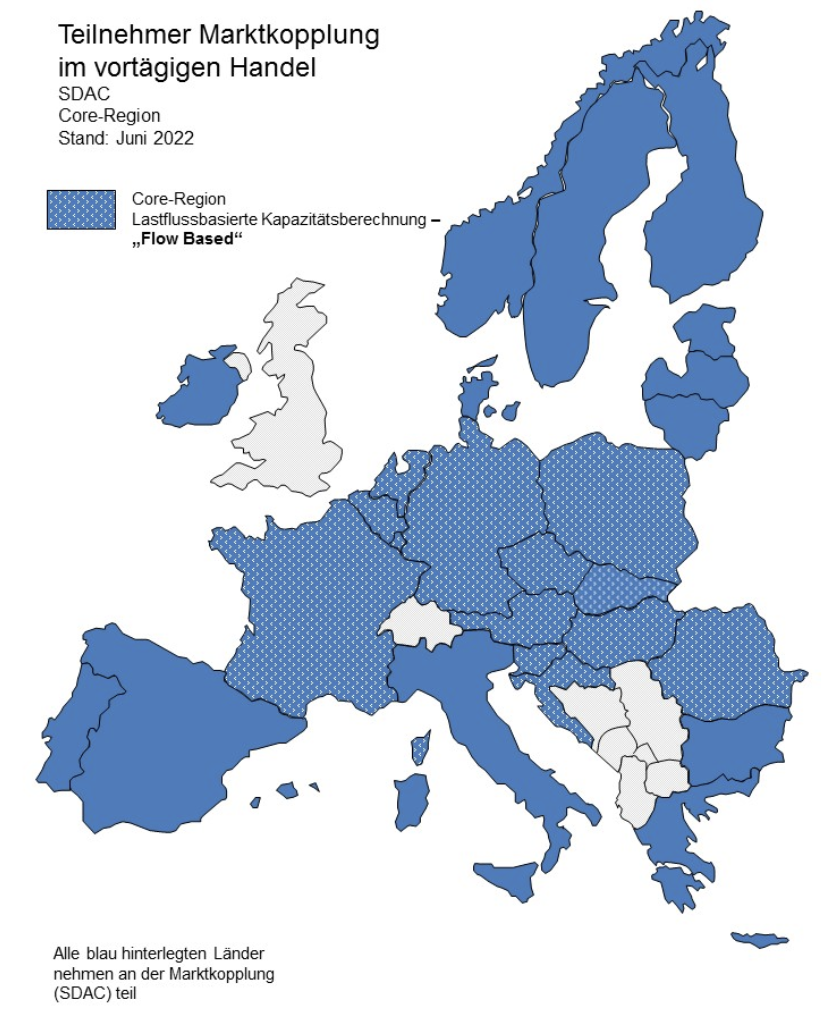
\includegraphics[width=0.5\textwidth]{Graphs/Abbildung1.png}}
    \caption{Karte mit SDAC- und FBMC-Ländern}
    \label{fig:Abbildung1}
\end{figure}

Im Juni 2022 stießen noch weitere osteuropäische Preiszonen hinzu, sodass es nunmehr 12 sind, die das FBMC verwenden (siehe Abbildung~\ref{fig:Abbildung1}).\\
Das Ziel des Market Couplings ist die Angleichung von Preisen. Abbildung~\ref{fig:Abbildung2} und \ref{fig:Abbildung3} zeigen ein Beispiel, das aus dem Paper von \cite{3} stammt, bestehend aus Preiszone A und Preiszone B. Beide Märkte befinden sich jeweils im Gleichgewicht mit einem niedrigeren eigenen Strompreis in Preiszone B und einem höheren  Preis in Preiszone A. Wenn nun von einer Austausch-Möglichkeit des Stroms ausgegangen wird, wird Strom aus Preiszone B von Preiszone A aufgekauft, da der Strom in Preiszone B günstiger ist als in A. Das resultiert in einem steigenden Angebot in Preiszone A, was dort den Preis sinken lässt. In Preiszone B hingegen sinkt das Angebot, da nun ein Teil des erzeugten Stroms dort nicht mehr am Markt ist. Der Preis steigt. Dieser Austausch geschieht so lange, bis sich beide Preise angeglichen haben. 

\begin{figure}[htbp]
    \centering
    % Erstes Bild
    \begin{minipage}{0.49\textwidth}
        \centering
        \href{https://www.tandfonline.com/doi/abs/10.1080/14697688.2020.1733059}{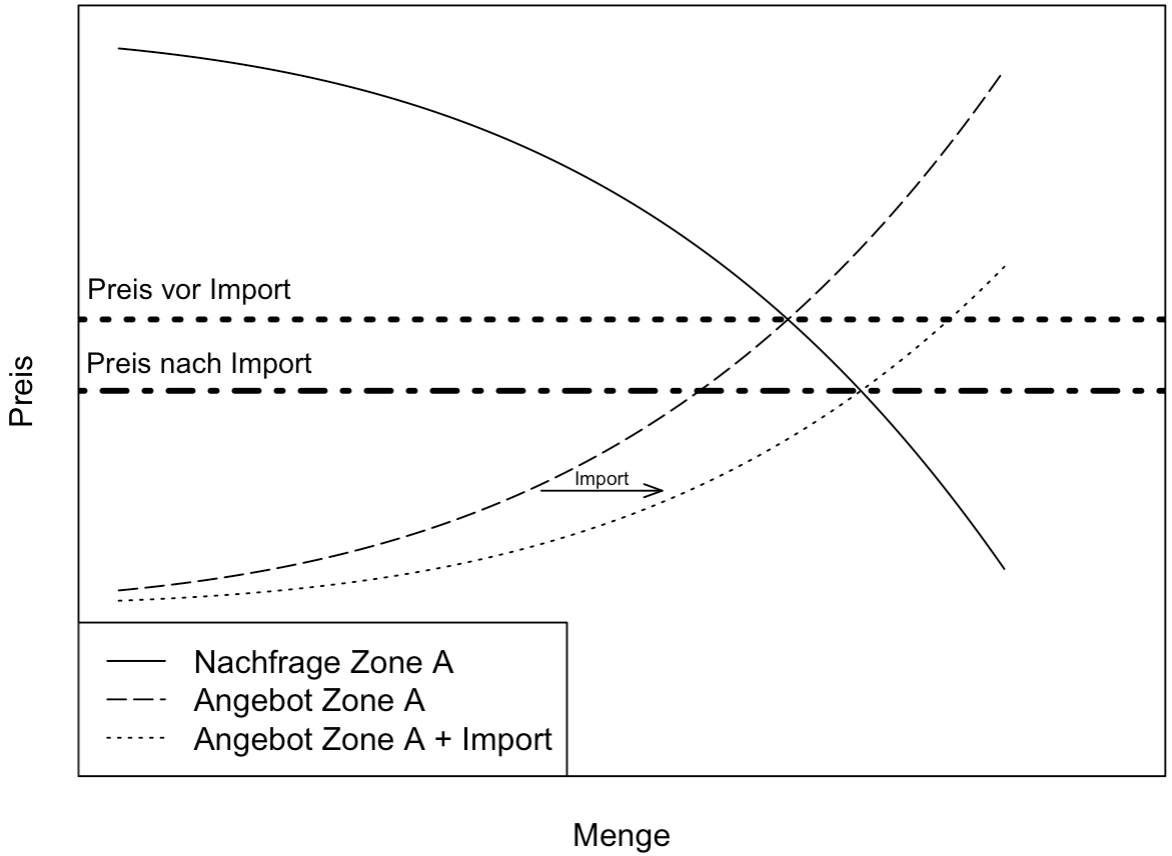
\includegraphics[width=\linewidth]{Graphs/Abbildung2.png}}
        \caption{Preiszone A}    
        \label{fig:Abbildung2}
    \end{minipage}
    \hfill
    % Zweites Bild
    \begin{minipage}{0.49\textwidth}
        \centering
        \href{https://www.tandfonline.com/doi/abs/10.1080/14697688.2020.1733059}{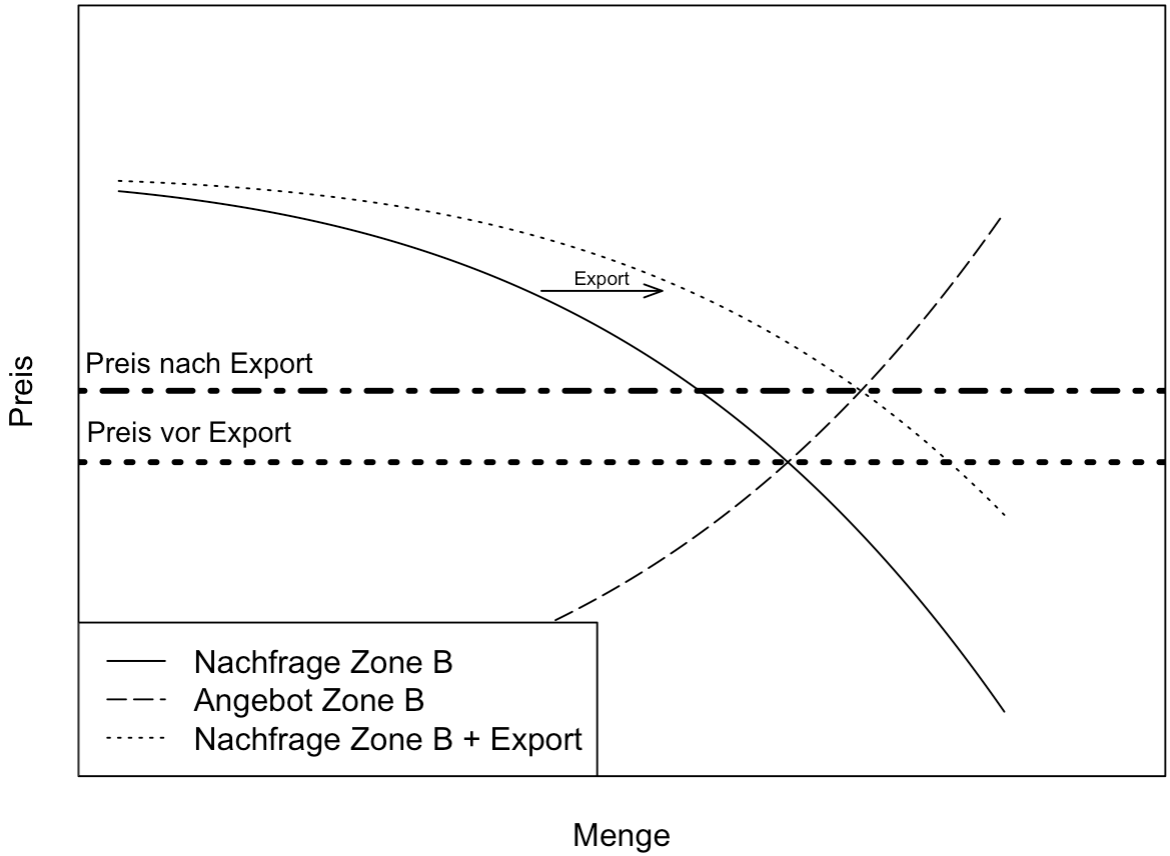
\includegraphics[width=\linewidth]{Graphs/Abbildung3.png}}
        \caption{Preiszone B}        
        \label{fig:Abbildung3}
    \end{minipage}
\end{figure}


\newpage
\subsection{Location Spreads}
\label{sec:Location Spreads}

Wenn der Austausch von Energie zwischen zwei Preiszonen nicht mehr in vollem Umfang möglich ist, gleichen sich die Preise in den Preiszonen nicht an und es entstehen Preisunterschiede (Price Spreads oder auch Location Spreads) durch lokale Preisbildung (\cite{3}). Dieser Austausch wird vor allem dann  behindert, wenn die physikalische Kapazität der grenzüberschreitenden Stromtrassen nicht ausreicht, um den Bedarf an Import oder Export zu decken.\footnote{Weitere seltene Ursachen, die aber im Verlauf der Arbeit nicht weiter untersucht werden, sind z.B. technische Probleme die zum (teilweisen) Ausfall des SDAC-Systems führen können , wie etwa am 28. Oktober 2023 \cite{ENTSOE_market_report}} \\
Für Marktakteure, insbesondere für Erzeuger erneuerbarer Energien (e.E.), sind Location Spreads von hoher Relevanz, denn das Wetter und somit auch die Erzeugung von Strom unterliegt großen Schwankungen. In Zeiten hoher Produktion aus Wind oder Photovoltaik kann es zu sehr niedrigen Preisen in Regionen mit hoher Erzeugung kommen, da durch den Merit-Order-Effekt diejenigen Erzeuger von Energien ins Netz einspeisen, die in der Produktion die geringsten Grenzkosten haben (\cite{7}).\\
Infolgedessen wird Strom in eine Preiszone exportiert, die einen höheren Strompreis hat. Sobald allerdings die Interkonnektoren-Kapazität ausgeschöpft ist, ist das nicht mehr möglich. Der Strom kann also nicht mehr exportiert werden und flutet nun den heimischen Markt. Der Umstand, dass bei gutem Wetter alle Erzeuger von e.E. gleichzeitig Strom in das Netz einspeisen, sorgt dafür, dass das Angebot in die Höhe schießt und dadurch der Preis enorm nach unten gedrückt wird. Die Betreiber von Anlagen mit e.E. erhalten also einen niedrigen Preis für ihren Strom und schaden sich gegenseitig. In der Literatur wird bei diesem Effekt, zum Beispiel in \cite{7} oder \cite{8}, vom Kannibalisierungseffekt (Cannibalization Effect) gesprochen. \\
Für Betreiber von e.E.-Anlagen ist es also wichtig, sich gegen diese Price Spreads abzusichern, damit sie auch bei einem sehr niedrigen Strompreis (wie im Falle einer Kannibalisierung) einen wirtschaftlich attraktiven Preis für ihren Strom erhalten. In der Literatur existieren verschiedene Analysen zu Price Spreads. \cite{10} betrachtet saisonale Trends und Sprünge zwischen zwei Ländern, \cite{12} versucht mit einem Copula-Modell und \cite{15} mit Monte-Carlo-Simulationen, Abhängigkeiten zwischen extremen Preisen zweier Preiszonen zu erklären. Es gibt auch Untersuchungen zu dem Gegenereignis, der Preis-Konvergenz. So verwendet \cite{13} etwa lineare Regression und \cite{16} Machine-Learning-Ansätze, um etwaige Muster zu erkennen\footnote{Das Modell von \cite{16} wird noch von \cite{20} mit Einbeziehung von e.E. verfeinert.}.



\newpage
\subsection{Vorstellung relevanter Finanzprodukte}
\label{sec:Vorstellung relevanter Finanzprodukte}
\begin{itemize}

    \item Indizes wie z.B. die von Speedwell Climate  (bspw. Quality Index) \textbf{1, 2}
    \item Je nachdem was am Ende in der Arbeit vorkommt Grundlagen zu diesen Produkten (-> kurze Erklärung zu Optionen, Power Future, Swaps) \textbf{4}
    
\end{itemize}
